\documentclass[10pt, a4paper]{article}

\usepackage{amssymb, amsmath}
\usepackage[utf8]{inputenc}
\usepackage[ngerman]{babel}
\usepackage{fancyhdr}
\usepackage{tikz}
\usepackage{fullpage}
\usepackage{graphicx}
\usepackage{alltt}
\pagestyle{fancy}
\setlength{\headheight}{12.4pt}
\setlength{\headsep}{1.5\headheight}

% 1. Person eintragen
\newcommand{\FirstAuthor}{Hasenauer}
\newcommand{\FirstAuthorFirstName}{Hannes}
\newcommand{\FirstAuthorMatnum}{**********}

% 2. Person eintragen
\newcommand{\SecAuthor}{Fritzsch}
\newcommand{\SecAuthorFirstName}{Daniel}
\newcommand{\SecAuthorMatnum}{0930754}

% 3. Person eintragen
\newcommand{\ThirdAuthor}{Temmel}
\newcommand{\ThirdAuthorFirstName}{Hans Christian}
\newcommand{\ThirdAuthorMatnum}{*********}

\newcommand{\AuthorFront}{{\normalsize
\begin{tabular}{|c|c|c|} \hline
\textbf{Nachname} & \textbf{Vorname}       & \textbf{Matrikelnummer} \\ \hline \hline
\FirstAuthor      & \FirstAuthorFirstName  & \FirstAuthorMatnum      \\ \hline
\SecAuthor        & \SecAuthorFirstName    & \SecAuthorMatnum        \\ \hline
\ThirdAuthor      & \ThirdAuthorFirstName  & \ThirdAuthorMatnum      \\ \hline
\end{tabular}}}

\author{\AuthorFront}
\newcommand{\Author}{\FirstAuthorMatnum, \SecAuthorMatnum,
                     \ThirdAuthorMatnum}

\date{} % Kein Datum angegeben
\fancyfoot{} % Seitenzahl unten nicht anzeigen

\lhead{Modern Information Systems}
\chead{\Author}
\rhead{Seite \thepage}

\title{Modern Information Systems WS 11/12}

\begin{document}

%%%%%%%%%%%%%%%%%%%%%%%%%%%%%%%%%%%%%%%%%%%%%%%%%%%%%%%%%%%%%%%%%%%%%%%%%%%%%%%%

\newcounter{ale}
\newcommand{\abc}{\item[\alph{ale})]\stepcounter{ale}}
\newenvironment{liste}{\begin{itemize}}{\end{itemize}}
\newcommand{\aliste}{\begin{liste} \setcounter{ale}{1}}
\newcommand{\zliste}{\end{liste}}
\newenvironment{abcliste}{\aliste}{\zliste}

%%%%%%%%%%%%%%%%%%%%%%%%%%%%%%%%%%%%%%%%%%%%%%%%%%%%%%%%%%%%%%%%%%%%%%%%%%%%%%%%

\maketitle
\thispagestyle{fancy}

%%%%%%%%%%%%%%%%%%%%%%%%%%%%%%%%%%%%%%%%%%%%%%%%%%%%%%%%%%%%%%%%%%%%%%%%%%%%%%%%

\tableofcontents
\pagebreak

\section{Database Schema}

\subsection{Entity-Relationship Diagram}

\begin{figure}[htb]
	\centering
	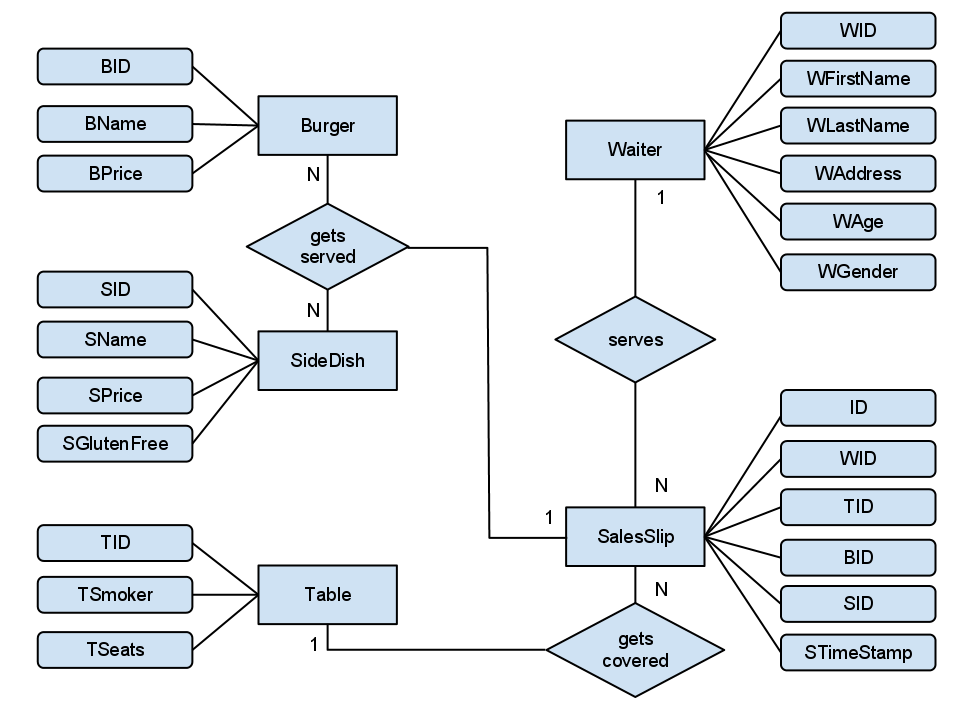
\includegraphics[scale=0.49]{fig/entity_relationship_diagram.png}
	\caption{Entity-Relationship Diagram}
\end{figure}

\subsection{Domains}

\begin{tabular}[ht]{| p{4.9cm} | p{4.9cm} | p{4.9cm} |}
\hline
  	Name 		& DataType 	& Description\\
\hline\hline
  	WID                	& Integer 		& Waiter ID\\
  	WFirstName 	& String   		& Firstname of the waiter\\
  	WLastName 	& String    		& Lastname of the waiter\\
 	WAddress    	& String    		& Address of the waiter\\
 	WAge           	& Integer   	& Age of the waiter\\
 	WGender     	& Integer   	& Gender of the waiter\\
\hline
  	TID                	& Integer   	& Table ID\\
  	TSmoker      	& Boolean	& Smokertable?\\
  	TSeats      		& Integer 		& Amount of seats\\
\hline
  	BID                	& Integer   	& Burger ID\\
  	BName      	& String		& Name of the burger\\
  	BPrice      		& Integer 		& Price of the burger\\
\hline
  	SID                	& Integer   	& Sidedish ID\\
  	SName      	& String		& Name of the sidedish\\
  	SPrice      		& Integer 		& Price of the sidedish\\
	SGlutenfree      	& Boolean 	& Glutenfree?\\
\hline
  	ID                	& Integer   	& Sales Slip ID\\
  	WID                	& Integer 		& Waiter ID\\
  	TID                	& Integer   	& Table ID\\
  	BID                	& Integer   	& Burger ID\\
  	SID                	& Integer   	& Sidedish ID\\
	STimeStamp    	& TimeStamp   	& The actual timestamp\\
\hline
\end{tabular}

\subsection{Relations}

\begin{tabular}[ht]{| p{2.8cm} | p{2.8cm} | p{2.8cm} | p{2.8cm} | p{2.8cm} |}
\hline
  	Waiter 			& Table 			& Burger			& SideDish 		& SalesSlip\\
\hline\hline
	\underline{WID}	& \underline{TID}     	& \underline{BID}	& \underline{SID}	& \underline{ID}\\
	WFirstName		& TSmoker     		& BName			& SName			& WID\\
	WLastName		& TSeats     		& BPrice			& SPrice			& TID\\
	WAddress			& 		     		&				& SGlutenFree		& BID\\
	WAge			& 		     		&				& 				& SID\\
	WGender			& 		     		&				& 				& STimeStamp\\
\hline
\end{tabular}

\subsubsection{Additional Description}

The domains WID, TID, BID and SID are the foreign keys in the relation SalesSlip.

\subsection{Functional Dependencies}

\begin{itemize}
	\item Waiter(\underline{WID}, WFirstName, WLastName, WAddress, WAge, WGender)
		\subitem - WID $\rightarrow$ WFirstName
		\subitem - WID $\rightarrow$ WLastName
		\subitem - WID $\rightarrow$ WAddress
		\subitem - WID $\rightarrow$ WAge
		\subitem - WID $\rightarrow$ WGender
	\item Table(\underline{TID}, TSmoker, TSeats)
		\subitem - TID $\rightarrow$ TSmoker
		\subitem - TID $\rightarrow$ TSeats
		
	\pagebreak	
	
	\item Burger(\underline{BID}, BName, BPrice)
		\subitem - 	BID $\rightarrow$ BName
		\subitem - 	BID $\rightarrow$ BPrice
	\item SideDish(\underline{SID}, SName, SPrice, SGlutenFree)
		\subitem - SID $\rightarrow$ SName
		\subitem - SID $\rightarrow$ SPrice
		\subitem - SID $\rightarrow$ SGlutenFree
	\item SalesSlip(\underline{ID}, WID, TID, BID, SID, STimeStamp)
		\subitem - ID $\rightarrow$ WID
		\subitem - ID $\rightarrow$ TID
		\subitem - ID $\rightarrow$ BID
		\subitem - ID $\rightarrow$ SID
		\subitem - ID $\rightarrow$ STimeStamp	
\end{itemize}

\subsubsection{Additional Description}

Every domain in the relation is only identifiable by a unique primary key. Therefore there are no indirect key dependencies and the database is in the 3rd normal form.

\pagebreak
\section{Practical Implementation}

\end{document}